\chapter{Einleitung}

\section{Was ist ein RAG}

\begin{figure}[h!]
    \centering
    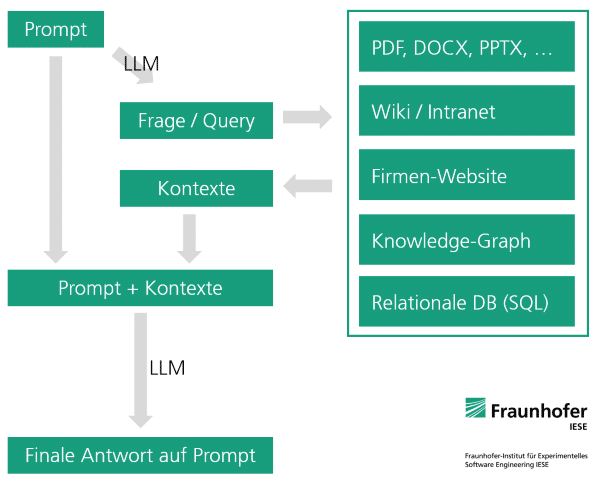
\includegraphics[width=0.5\textwidth]{retrieval_augmented_generation_RAG_600px.png}
    \caption{Stuktur eines RAGS, Quelle: \cite{honroth2024retrieval}}
    \label{fig:Rag Structure}
\end{figure}

\begin{quote}
    Bei Retrieval Augmented Generation (RAG) erweitert man den Prompt für das Large Language Model um Suchergebnisse aus einer Dokumentensammlung, einer Datenbank, einem Wissensgraph (Knowledge Graph) oder einer anderen Suche (z.B. Internetsuche). Das Wissen für die Antwort kommt also aus angebundenen Quellen und nicht aus dem LLM.
\end{quote}
\cite{honroth2024retrieval}\\ \\

Die nutzung eines RAGs ist eine der beiden Möglichkeiten, um ein LLM zu verbessern. Die andere Möglichkeit ist das Fine-Tuning des LLMs, es gibt jedoch wichtige Unterscheide zwischen diesen beiden Methoden.

Es gibt einige Faktoren welche die Entscheidung beeinflussen können, ob ein RAG oder ein Fine-Tuning besser für den betrieblichen Ablauf geeignet ist.

\subsection{Kompetenz}
Beim Fine-Tuning ist ein gewisses technisches Wissen notwendig, um die Themen Natural Language Processing (NLP), Deep Learning, Modellkonfiguration, Datenaufbereitung und Evaluierung an zu wenden.
Der gesammte Prozess des Fine-Tunings ist sehr komplex und erfordert viel Zeit und Ressourcen.

\subsection{Art der Daten}
Sollten die Daten Dynamisch sein, ist das RAG die bessere Lösung, da es die Daten schneller und kontinuierlich aktualisieren kann.
Der Prozess des Fine-Tunings erstellt immer eine Snapshot der ein erneutes Training erfordert.
Beim Fine-tuning ist es möglich, dass das Modell Muster erkennt und Firmen eigene Begriffe verstehen kann.

\subsection{Budget}
Das Fine-Tuning benötigt tuere Rechenzeit auf hochleistungs GPUs, das macht das training eines Modells sehr teuer.
Das RAG hat dagegen zusätliche Kosten die durch das Speichern der Daten in einer Vektordatenbank entstehen.


\section{Objektive Beurteilung von RAGs}
Desto mehr Daten einem RAG zur Verfügung stehen, desto aufwendiger ist es die Qualität des RAGs zu beurteilen.
Eine beurteilung durch menschen müsste bei Anpassungen am RAG oder Änderungen an den Daten immer wieder neu durchgeführt werden.
Menschliche Beurteilungen sind teurer, daher ist es ergibt es Sinn, mithilfe von LLMs die Beurteilung zu automatisieren.
Es gibt bereits tools wie RAGAs die versuchen diesen Prozess unter anderem mithilfe von LLMs zu automatisieren.
Diese Tools generieren aus den ihnen gegebenen Daten Fragebögen, die auf eine Frage eine beispielhafte Antwort und die genutzten Stellen aus den vorher gegebenen Dokumenten beinhalten.
Sollten nach diesem autmatisierten Test die gewünschten Ergebnisse nicht erreicht werden können zum Beispiel Veröffentlichung blockiert werden.

Sowohl menschlich Bewertungen als auch die reine subjektive Bewertung durch LLMs sind nicht objektiv.
Mithilfe von mehreren Techniken kann versucht werden die Bewertung mithilfe von LLMs objektiv zu machen.

\section{Darstellung des Themas und der Forschungsfragen}
In dieser Bachelorarbeit wird untersucht, wie gut diese Tools sowohl subjektive als auch objektive Bewertungen durchführen können.
Im Mitelpunkt werden die beiden Tools RAGAS und Gistkard stehen, welche die Bewertung durchführen.




\section{Praxistauglichkeit und Herausforderungen}
Es stellen sich mehrere Herausforderungen für die Bewertung von RAGs durch diese Tools.
Der erste ist die die Kosten die bei der Bewertung entstehen, für die Bewertung muss das neue System welches getestet werden aufgesetzt werden.
Dies beinhaltet eine eventuelle doppelte Speicherung der Daten und die für das Testen benötigten Aufrufe des LLMs.
Neben den Kosten ist auch die Zeit welche es dauert die Bewertung durch zu führen relevant, da die Bewertung schneller durchgeführt werden kann, wenn mehr Ressourcen zur Verfügung stehen.
Das System muss auch auf dem neusten Stand gehalten werden, da sich diese noch realtiv junge Thema schnell entwickelt.

Content filtering

\section{Softwaretechnische Fragestellungen}

Fehler beim generieren https://pixion.co/blog/rag-in-practice-test-set-generation

LLM positional bias https://arxiv.org/pdf/2305.17926

Pitfalls in LLM Assisted Evaluation https://medium.aiplanet.com/evaluate-rag-pipeline-using-ragas-fbdd8dd466c1

Rate Limits

Sind RAGS bald tod?
https://x.com/agishaun/status/1758561862764122191
https://x.com/ptsi/status/1758511315646320920
